\documentclass{amsart}
\usepackage{graphicx}
\usepackage{epstopdf}
\usepackage{epsfig}
%
\begin{document}
%
\begin{center}
Notes on Artificial Neural Networks
\end{center}
%
\begin{figure}[h!]
\label{colliding_spheres}
\centering
  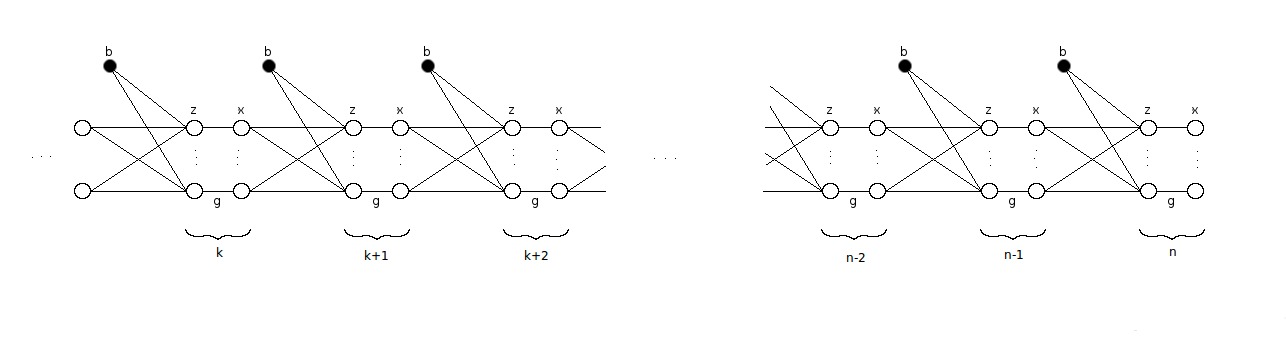
\includegraphics[angle=0,width=140mm]{ANN.jpg}
\caption{ANN}
\end{figure}
%
\begin{equation*}
z_q^{k+1} = \sum_{i=0}^{N^k} x_i^k w_{i,q}^k + v_q^k b
\end{equation*}
%
\begin{equation*}
E = \frac{1}{2} \sum_{i=0}^N (x_i^n - t_i)^2
\end{equation*}
%
\begin{equation*}
\begin{aligned}
&\frac{\partial E}{\partial \omega_{p,q}^k} = \sum_{i_n = 0}^{N^n} \Bigg( \frac{\partial E}{\partial x_{i_n}^n}
\frac{\partial x_{i_n}^n}{\partial g} \frac{\partial g}{\partial z_{i_n}^n} \sum_{i_{n-1}=0}^{N^{n-1}} \Bigg(
\frac{\partial z_{i_n}^n}{\partial x_{i_{n-1}}^{n-1}} \frac{\partial x_{i_{n-1}}^{n-1}}{\partial g}
\frac{\partial g}{\partial z_{i_{n-1}}^{n-1}} \Bigg( \sum_{i_{n-2}=0}^{N^{n-2}}
\frac{\partial z_{i_{n-1}}^{n-1}}{\partial x_{i_{n-2}}^{n-2}}
\frac{\partial x_{i_{n-2}}^{n-2}}{\partial g} \frac{\partial g}{\partial z_{i_{n-2}}^{n-2}}
\sum_{i_{n-3}=0}^{N^{n-3}} \Bigg( \ldots\\
&\ldots \sum_{i_{k+2}=0}^{N^{k+2}} \Bigg( \frac{\partial z_{i_{k+3}}^{k+3}}{\partial x_{i_{k+2}}^{k+2}}
\frac{\partial x_{i_{k+2}}^{k+2}}{\partial g}
\frac{\partial g}{\partial z_{k+2}^{k+2}} \Bigg( \frac{\partial z_{i_{k+2}}^{k+2}}{\partial x_p^{k+1}}
\frac{\partial x_p^{k+1}}{\partial g}
\frac{\partial g}{\partial z_p^{k+1}} \Bigg(
\frac{\partial z_p^{k+1}}{\partial \omega_{p,q}^k} \Bigg)\Bigg)\Bigg)\Bigg) \ldots \Bigg)\Bigg)\Bigg)\Bigg)
\end{aligned}
\end{equation*}
%
And the bias weights $v$ come out with the same process:
%
\begin{equation*}
\begin{aligned}
&\frac{\partial E}{\partial v_q^k} = \sum_{i_n = 0}^{N^n} \Bigg( \frac{\partial E}{\partial x_{i_n}^n}
\frac{\partial x_{i_n}^n}{\partial g} \frac{\partial g}{\partial z_{i_n}^n} \sum_{i_{n-1}=0}^{N^{n-1}} \Bigg(
\frac{\partial z_{i_n}^n}{\partial x_{i_{n-1}}^{n-1}} \frac{\partial x_{i_{n-1}}^{n-1}}{\partial g}
\frac{\partial g}{\partial z_{i_{n-1}}^{n-1}} \Bigg( \sum_{i_{n-2}=0}^{N^{n-2}}
\frac{\partial z_{i_{n-1}}^{n-1}}{\partial x_{i_{n-2}}^{n-2}}
\frac{\partial x_{i_{n-2}}^{n-2}}{\partial g} \frac{\partial g}{\partial z_{i_{n-2}}^{n-2}}
\sum_{i_{n-3}=0}^{N^{n-3}} \Bigg( \ldots\\
&\ldots \sum_{i_{k+2}=0}^{N^{k+2}} \Bigg( \frac{\partial z_{i_{k+3}}^{k+3}}{\partial x_{i_{k+2}}^{k+2}}
\frac{\partial x_{i_{k+2}}^{k+2}}{\partial g}
\frac{\partial g}{\partial z_{k+2}^{k+2}} \Bigg( \frac{\partial z_{i_{k+2}}^{k+2}}{\partial x_p^{k+1}}
\frac{\partial x_p^{k+1}}{\partial g}
\frac{\partial g}{\partial z_p^{k+1}} \Bigg(
\frac{\partial z_p^{k+1}}{\partial v_p^k} \Bigg)\Bigg)\Bigg)\Bigg) \ldots \Bigg)\Bigg)\Bigg)\Bigg)
\end{aligned}
\end{equation*}
%
\begin{equation*}
\frac{\partial E}{\partial x_i} = (x_i^n - t_i)
\end{equation*}
%
\begin{equation*}
\frac{\partial z_q^{k+1}}{\partial \omega_{p,q}^k} = x_p^k
\end{equation*}
%
\begin{equation*}
\frac{\partial z_q^{k+1}}{\partial v_q^k} = b
\end{equation*}
%
\begin{equation*}
\frac{\partial z_{i_n}^{n}}{\partial x_{i_{n-1}}^{n-1}} = \omega_{i_{n},i_{n-1}}^{n-1}
\end{equation*}
%
\begin{equation*}
\frac{\partial x}{g} = 1
\end{equation*}
%
\begin{equation*}
x^k = g(z^k;\beta) = \frac{1}{1 + exp(-\beta z^k )}
\end{equation*}
%
\begin{equation*}
D_g(z^k;\beta) = \frac{\partial g}{\partial z^k} = \beta \frac{\exp(-\beta z^k)}{(1 + \exp(-\beta z^k))^2} = \beta g(z^k; \beta) \big( 1 - g(z^k; \beta)) = \beta x^k (1 - x^k)
\end{equation*}
%
Then making these substitutions:
%
\begin{equation*}
\begin{aligned}
&\frac{\partial E}{\partial \omega_{p,q}^k} = \sum_{i_{k+2}=0}^{N^{k+2}} \Bigg (
(x_i^n - t_i) D_g(z_{i_n}^n;\beta) \sum_{i_{n-1}=0}^{N^{n-1}} \Bigg ( \omega_{i_{n},i_{n-1}}^{n-1} D_g(z_{i_{n-1}}^{n-1};\beta)
\sum_{i_{n-2}=0}^{N^{n-2}} \Bigg ( \omega_{i_{n-1},i_{n-2}}^{n-2} D_g ( z_{i_{n-2}}^{n-2};\beta )
\sum_{i_{n-3}=0}^{N^{n-3}} \Bigg ( \ldots\\
&\ldots \sum_{i_{k+2}=0}^{N^{k+2}} \Bigg ( \omega_{i_{k+3},i_{k+2}}^{k+2} D_g (z_{i_{k+2}}^{k+2};\beta) \Bigg ( \omega_{i_{k+2},p}^{k+1}
D_g (z_p^{k+1};\beta) x_q^k \Bigg )\Bigg )\Bigg )\Bigg ) \ldots \Bigg )\Bigg )\Bigg )\Bigg )
\end{aligned}
\end{equation*}
%
\begin{equation*}
\begin{aligned}
&\frac{\partial E}{\partial \omega_{p,q}^k} = \sum_{i_{k+2}=0}^{N^{k+2}} \Bigg (
(x_i^n - t_i) \beta x_{i_n}^n (1 - x_{i_n}^n) \sum_{i_{n-1}=0}^{N^{n-1}} \Bigg ( \omega_{i_{n},i_{n-1}}^{n-1} \beta x_{i_{n-1}}^{n-1} (1 - x_{i_{n-1}}^{n-1})
\sum_{i_{n-2}=0}^{N^{n-2}} \Bigg ( \omega_{i_{n-1},i_{n-2}}^{n-2} \beta x_{i_{n-2}}^{n-2} (1 - x_{i_{n-2}}^{n-2})
\sum_{i_{n-3}=0}^{N^{n-3}} \Bigg ( \ldots\\
&\ldots \sum_{i_{k+2}=0}^{N^{k+2}} \Bigg ( \omega_{i_{k+3},i_{k+2}}^{k+2} \beta x_{i_{k+2}}^{k+2} (1 - x_{i_{k+2}}^{k+2}) \Bigg ( \omega_{i_{k+2},p}^{k+1}
\beta x_p^{k+1} (1 - x_p^{k+1}) x_q^k \Bigg )\Bigg )\Bigg )\Bigg ) \ldots \Bigg )\Bigg )\Bigg )\Bigg )
\end{aligned}
\end{equation*}
%
\begin{equation}
\label{longSum}
\begin{aligned}
&\frac{\partial E}{\partial \omega_{p,q}^k} = \sum_{i_{k+2}=0}^{N^{k+2}} \Bigg (
(x_i^n - t_i) \beta x_{i_n}^n (1 - x_{i_n}^n) \sum_{i_{n-1}=0}^{N^{n-1}} \Bigg ( \omega_{i_{n},i_{n-1}}^{n-1} \beta x_{i_{n-1}}^{n-1} (1 - x_{i_{n-1}}^{n-1})
\sum_{i_{n-2}=0}^{N^{n-2}} \Bigg ( \omega_{i_{n-1},i_{n-2}}^{n-2} \beta x_{i_{n-2}}^{n-2} (1 - x_{i_{n-2}}^{n-2})
\sum_{i_{n-3}=0}^{N^{n-3}} \Bigg ( \ldots\\
&\ldots \sum_{i_{k+2}=0}^{N^{k+2}} \Bigg ( \omega_{i_{k+3},i_{k+2}}^{k+2} \beta x_{i_{k+2}}^{k+2} (1 - x_{i_{k+2}}^{k+2}) \Bigg ( \omega_{i_{k+2},p}^{k+1}
\beta x_p^{k+1} (1 - x_p^{k+1}) x_q^k \Bigg )\Bigg )\Bigg )\Bigg ) \ldots \Bigg )\Bigg )\Bigg )\Bigg )
\end{aligned}
\end{equation}
%
The weights are updated as follows:
%
\begin{equation*}
\omega_{p,q}^k - \eta \frac{\partial E}{\partial \omega_{p,q}^k} \rightarrow \omega_{p,q}^k
\end{equation*}
%
where $\eta$ is the learning rate.
%
%%%%%%%%%%%%%%%%%%%%%%%%%%%%%%%%%%%
%%%%%%%%% 3 layers %%%%%%%%%%%%%%%%
%%%%%%%%%%%%%%%%%%%%%%%%%%%%%%%%%%%
%
In the case of three layers, either three layers deep in the network or the network is only three layers in length,
%
\begin{equation*}
\frac{\partial E}{\partial \omega_{p,q}^{n-2}} = \sum_{i_n=0}^{N^n} \Bigg( (x_{i_n}^n - t_{i_n}) D_g(z_{i_n}^n; \beta) \Bigg( \omega_{{i_n},i_p}^{n-1} D_g(z_p^{n-1};\beta) x_q^{n-2} \Bigg) \Bigg)
\end{equation*}
%
For only two layers, either the network is two layers deep or we are only looking at the set of weights at the end of the network:
%
\begin{equation*}
\frac{\partial E}{\partial w_{p,q}^{n-1}} = (x_p^{n} - t_p) D_g(z_p^{n};\beta) x_q^{n-1}.
\end{equation*}
%%%%%%%%%%%%%%%%%%%%%%%%%%%%%%%%%%%%
%%%% simplification %%%%%%%%%%%%%%%%
%%%%%%%%%%%%%%%%%%%%%%%%%%%%%%%%%%%%
%
\newpage
Define
%
\begin{equation}
\label{definitions}
\begin{aligned}
&A^k := D_g(z^{k+1};\beta) \otimes x^k = \big(\beta x^{k+1} \circ (1 - x^{k+1}) \big) \otimes x^k\\
&\varpi_{i,j}^k := \omega_{i,j}^k D_g(z_j^k) = \omega_{i,j}^k \big( \beta x_j^k (1 - x_j^k)) \big)\\
&W^k := \varpi^{n-1} \varpi^{n-2} \cdots \varpi^k \Rightarrow W^k = W^{k+1} \varpi^k\\
&\Delta := (x^n - t) \circ D_g(z^n) = (x^n - t) \circ \big( \beta x^n \circ (1 - x^n) \big)
\end{aligned}
\end{equation}
%
Then \eqref{longSum} becomes
%
\begin{equation}
\label{shortSum}
\begin{aligned}
\frac{\partial E}{\partial \omega_{p,q}^k} = &\sum_{i_n=0}^{N^n} \Bigg( \Delta_{i_n} \sum_{i_{n-1}=0}^{N^{n-1}} \Bigg(\varpi_{i_n,i_{n-1}}^{n-1} \sum_{i_{n-2}=0}^{N^{n-2}} \Bigg(\varpi_{i_{n-1},i_{n-2}}^{n-2} \sum_{i_{n-3}=0}^{N^{n-3}} \Bigg( \ldots\\
&\sum_{i_{k+2}=0}^{N^{k+2}} \Bigg(\varpi_{i_{k+3},i_{k+2}}^{k+2} \Bigg(\omega_{i_{k+2},p}^{k+1} a_{p,q}^{k+1} \Bigg)\Bigg)\Bigg)\Bigg) \ldots \Bigg)\Bigg)\Bigg)\Bigg).
\end{aligned}
\end{equation}
%
re-writing \eqref{shortSum} using \eqref{definitions} and matrix notation:
%
\begin{equation*}
\frac{\partial E}{\partial \omega^k} = 
\left [
\left (
\begin{array}{ccc}
\Delta_1 & \cdots & \Delta_{N^n} \\
\vdots & \vdots & \vdots \\
\Delta_1 & \cdots & \Delta_{N^n} \\
\end{array}
\right )
W^{k+2} \omega^{k+1}
\right]^T \circ A^k
\end{equation*}
%
Then
%
\begin{equation*}
\omega^k - \eta \frac{\partial E}{\partial \omega^k} \rightarrow \omega^k
\end{equation*}
%
and
%
\begin{equation*}
\frac{\partial E}{\partial v^k} = 
\left [
\left (
\begin{array}{ccc}
\Delta_1 & \cdots & \Delta_{N^n} \\
\vdots & \vdots & \vdots \\
\Delta_1 & \cdots & \Delta_{N^n} \\
\end{array}
\right )
W^{k+2} \omega^{k+1}
\right]^T \circ \big(x^{k+1} \circ (1 - x^{k+1}) \big) b
\end{equation*}
%
Then
%
\begin{equation*}
v^k - \eta \frac{\partial E}{\partial v^k} \rightarrow v^k
\end{equation*}
%
For 3 layers:
%
\begin{equation*}
\frac{\partial E}{\partial \omega^{n-2}} = 
\left [
\left (
\begin{array}{ccc}
\Delta_1 & \cdots & \Delta_{N^n} \\
\vdots & \vdots & \vdots \\
\Delta_1 & \cdots & \Delta_{N^n} \\
\end{array}
\right ) \omega^{n-1}
\right ]^T
\circ A^{n-2}
\end{equation*}
%
And for 2 layers:
%
\begin{equation*}
\frac{\partial E}{\partial \omega^{n-1}} = 
\left (
\begin{array}{ccc}
\Delta_1 & \cdots & \Delta_{N^n} \\
\vdots & \vdots & \vdots \\
\Delta_1 & \cdots & \Delta_{N^n} \\
\end{array}
\right )^T
\circ A^{n-1}
\end{equation*}
%
\end{document}
